\section{Experimental Evaluation}
\label{sec:exp}

The practical part of this work focuses on comparison of the models presented in the previous section.
As the main goal of this study is to determine tighter bounds, the conducted experiments are designed for this purpose.
Instances of intended number of vertices are generated with random coordinates uniformly distributed between [0, 0] and [100, 100].
All computations were made on an Intel Core 2 Quad CPU at 2.83 GHz and 8 GB RAM.
The models were implemented in Java with Concert technology and solved using CPLEX 12.5.1 optimizer.
 
%\subsection{Instance generation}
\subsection{Comparison of the models}

The first experimental settings gives an overview of the studied models with respect to their strength and computational time.

\begin{table}[h!]
\centering
\setlength{\tabcolsep}{6pt} % Default value: 6pt
\renewcommand{\arraystretch}{1.4} % Default value: 1
\begin{tabular}{rrrrrrrr}
$|V|$ & $|D|$ & $LP(\mathcal{X}_1)$ & $LP(\mathcal{F}_1)$ & $LP(\mathcal{X}_2)$ & $LP(\mathcal{F}_2)$ & $LP(\mathcal{X}_3)$ &$LP(\mathcal{F}_3)$\\\hline
  16 & 8       & 70.29  & 79.96  & 80.82    & 85.19    & 99.58  & 99.58\\
  18 & 9       & 65.68  & 77.17  & 74.48    & 79.84    & 99.70  & 74.17\\ 
\end{tabular}
\caption{Average proportion of the optimal value calculated from 25 instances}
\label{tab:small_inst_cost}
\end{table}

\begin{table}[h!]
\centering
\setlength{\tabcolsep}{6pt} % Default value: 6pt
\renewcommand{\arraystretch}{1.4} % Default value: 1
\begin{tabular}{rrrrrrrrr}
 $|V|$ & $|D|$ & $LP(\mathcal{X}_1)$ & $LP(\mathcal{F}_1)$ & $LP(\mathcal{X}_2)$ & $LP(\mathcal{F}_2)$ & $LP(\mathcal{X}_3)$ & $LP(\mathcal{F}_3)$ & $\mathcal{F}_1$\\ \hline
  16 & 8       & 0.72   & 0.76   & 0.92     & 0.92     & 70.56  & 306.44  & 18.96 \\
  18 & 9       & 1.29   & 1.96   & 1.96     & 2.41     & 325.54 & 1139.92 & 65.29\\ 
\end{tabular}
\caption{Comparison of average runtime in seconds}
\label{tab:small_inst_time}
\end{table}

\subsection{Experiments on small instances}

Small instances can often be solved to optimality relatively quickly with branch and bound (B\&B).
We investigate what is the maximum size of instances that can be solved to optimality within 20 minutes using models $\mathcal{X}_1$ and $\mathcal{F}_1$.
The experiments compare sets of instances with different $|V|/|D|$ ratio.
Each value in Tab. \ref{tab:small_inst} was obtained after solving 25 instances with given numbers of destinations and non-destinations.
 
\begin{table}[h!]
\centering
\setlength{\tabcolsep}{12pt} % Default value: 6pt
\renewcommand{\arraystretch}{1.4} % Default value: 1
\begin{tabular}{rrrrrrrr}
  ~ & ~ & \multicolumn{2}{c}{average time [s]} &\multicolumn{2}{c}{\# solved} &\multicolumn{2}{c}{\shortstack{average \\remaining gap[\%]}}\\ \hline
 $|V|$ & $|D|$ & $\mathcal{F}_1$   & $\mathcal{X}_1$   & $\mathcal{F}_1$ & $\mathcal{X}_1$ & $\mathcal{F}_1$ & $\mathcal{X}_1$\\ \hline
  18 & 12      & 84   & 139  & 25 & 24 & 0.00  & 0.52\\
  21 & 14      & 789  & 1006 & 18 & 10 & 5.08  & 9.64\\ 
  24 & 16      & 1137 & 1161 & 4  & 3  & 20.52 & 21.04\\ \hline 
 %27 & 18 & ~ & ~ & ~ & ~ & ~ & ~\\  
 20 & 10 & 190 & 387 & 25 & 21 & 0.00 & 3.00 \\
  22 & 11 & 637 & 880 & 22 & 14 & 0.64 & 7.16\\
  24 & 12 & 997 & 1169 & 10 & 3 & 10.44 & 16.44\\ \hline
 % 26 & 13 & 1189 & 1200 & 1 & 0 & ~ & ~\\ \hline
  21 & 7 & 113 & 282 & 25 & 21 & 0.00 & 2.56\\ 
  24 & 8 & 442 & 650 & 21 & 16 & 2.72 & 8.64\\ 
  27 & 9 & 1013 & 1146 & 8 & 4 & 14.64 & 22.80\\ 
\end{tabular}
\caption{Computational results of Branch and bound on small instances}
\label{tab:small_inst}
\end{table}

\subsection{Experiments on medium size instances}

When it is not possible to solve integer models within the given time limit, we pursue lower bounds obtained by solving LP relaxations of the models.
We want to get as strong lower bound as possible, but as shown in the previous sections, LP relaxations of the strongest models have worse runtime than basic IP models, and at this point the constraint generation scheme comes into play.
Using this method, it is possible to get strong lower bounds quickly, often even an integral solution.

B\&B also produces LP relaxation during its course, and even though the computation is interrupted before the optimum is found, it is possible to keep track of the best bound at any moment of the computation.
We compare the progress of objective value obtained by the CG method and the best lower bound found by applying B\&B to $\mathcal{F}_1$ a restricted amount of time.
 
The values in the graphs represent a mean percentage of an objective value yielded by LP($\mathcal{F}_1$).
The values are calculated from 5 instances.
 
\begin{figure}[!htb]
    \centering
    \begin{subfigure}[b]{0.49\textwidth}
        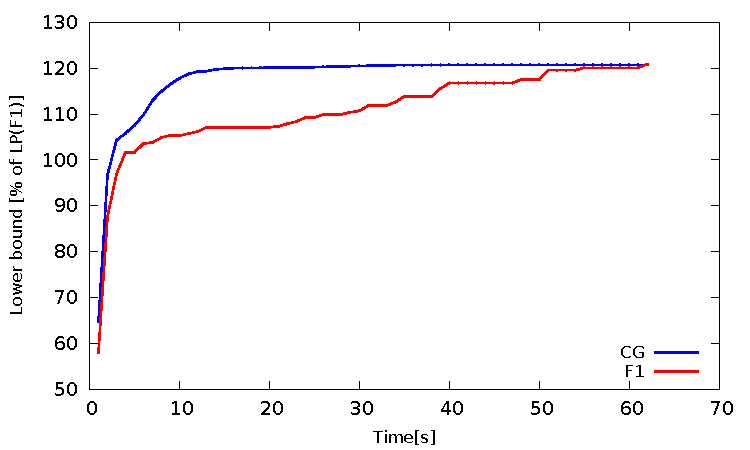
\includegraphics[width=\textwidth]{lower-bound-18-9}
        \caption{$|V|=18, |D|=9$}
        \label{fig:cggr18-9}
    \end{subfigure}
    \hfill %add desired spacing between images, e. g. ~, \quad, \qquad, \hfill etc. 
      %(or a blank line to force the subfigure onto a new line)
    \begin{subfigure}[b]{0.49\textwidth}
        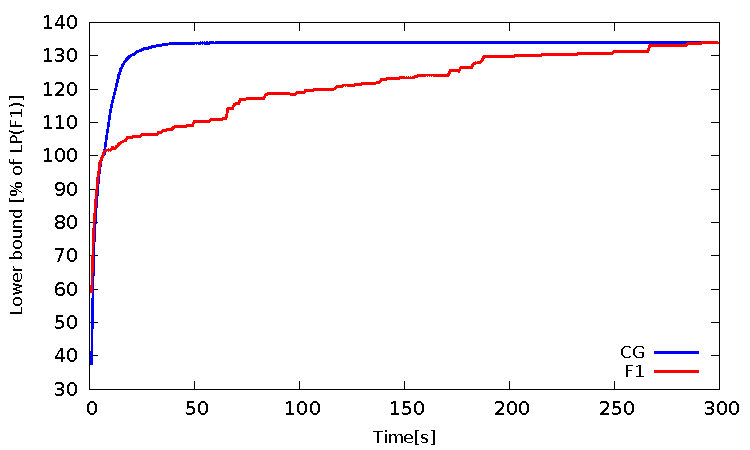
\includegraphics[width=\textwidth]{lower-bound-20-10}
        \caption{$|V|=20, |D|=10$}
        \label{fig:cggr20-10}
    \end{subfigure}
  
    \begin{subfigure}[b]{0.49\textwidth}
        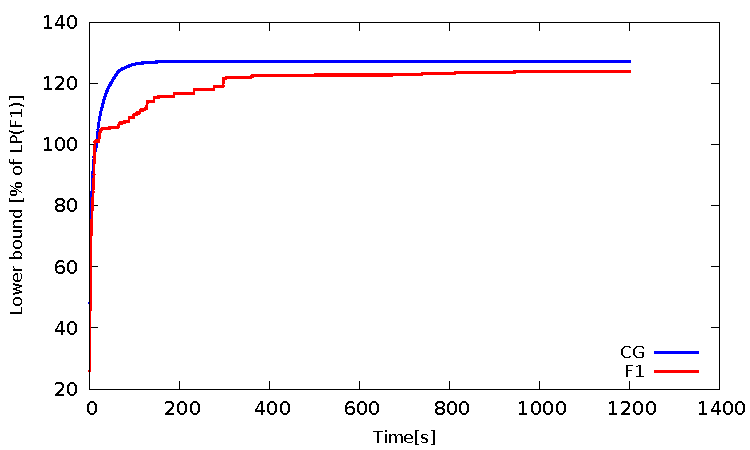
\includegraphics[width=\textwidth]{lower-bound-22-11}
        \caption{$|V|=22, |D|=11$}
        \label{fig:cggr22-11}
    \end{subfigure}
    \hfill %add desired spacing between images, e. g. ~, \quad, \qquad, \hfill etc. 
      %(or a blank line to force the subfigure onto a new line)
    \begin{subfigure}[b]{0.49\textwidth}
        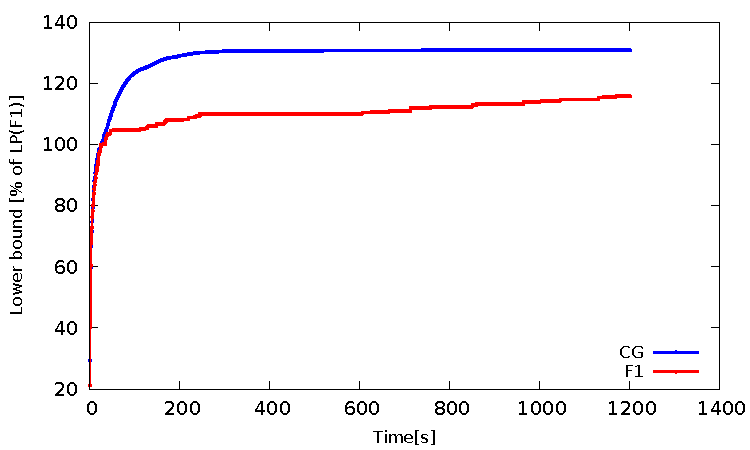
\includegraphics[width=\textwidth]{lower-bound-24-12}
        \caption{$|V|=24, |D|=13$}
        \label{fig:cggr24-12}
    \end{subfigure}

    \begin{subfigure}[b]{0.49\textwidth}
        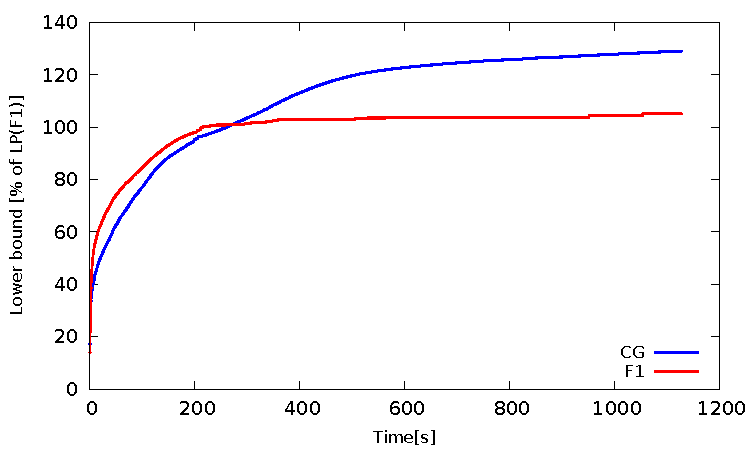
\includegraphics[width=\textwidth]{lower-bound-30-15}
        \caption{$|V|=30, |D|=15$}
        \label{fig:cggr30-15}
    \end{subfigure}
    \hfill %add desired spacing between images, e. g. ~, \quad, \qquad, \hfill etc. 
      %(or a blank line to force the subfigure onto a new line)
    \begin{subfigure}[b]{0.49\textwidth}
        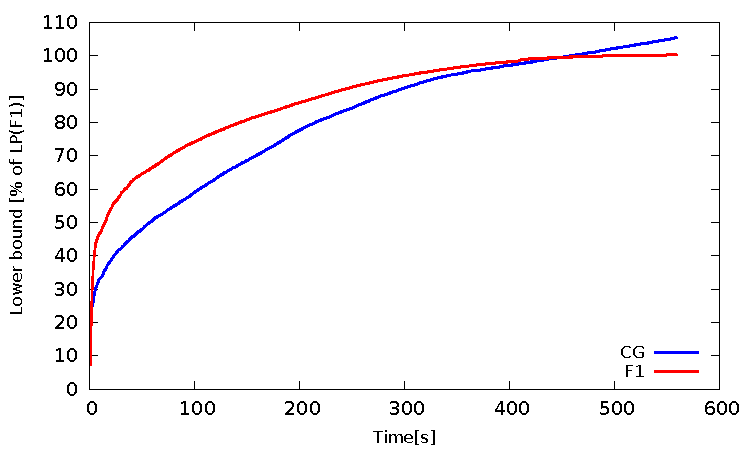
\includegraphics[width=\textwidth]{lower-bound-32-16}
        \caption{$|V|=32, |D|=16$}
        \label{fig:cggr32-16}
    \end{subfigure}
  \caption{Comparison of lower bound obtained by constraint generation and branch and bound on model $\mathcal{F}_1$. } \label{fig:cggr}
\end{figure} 

It is clear from the graphs that constraint generation is a suitable method for obtaining a lower bound for instances that cannot be solved to optimality using B\&B. CG provides a tighter bound at any time step of the computation.

\subsection{Experiments on large instances}

For instances in which $\mathcal{X}_3$ cannot be solved by CG within the given time limit, we investigate the best lower bounds that can be achieved by solving the LP relaxations of the weaker models.
